\cotefile{82}
\scanpage{17}
% lines 1–2
\deleted{produit scalaire avec $z\in\Gamma_S(E)$, et poser $z'={}^tf(z)$}

% lines 3
\[
\deleted{\langle\rho_E(\xi')\mathbin{.}x,z'\rangle=\deleted{\unsure{f}}\langle\alpha'(x'\wedge f(x)),z'\rangle}
\]

% lines 4–5
\deleted{ou \unsure{encore|exige}} $f(\rho_E(\xi')\mathbin{.}x)=f(\alpha'(\xi'\wedge f(x)))$ elle résulte \deleted{\unsure{$\rho_E$}} de la formule plus précise

% lines 6
\[
\rho_E(\xi')\mathbin{.}x=\alpha'(\xi'\wedge f(x)) \tag*{(56 bis)}
\]

% lines 7–9
qui, s'écrit, en prenant le produit scalaire avec $x'$ dans $E'$ et explicitant le premier membre grâce à (59 bis)

% lines 10–13
\[
\begin{aligned}
-\langle x,[\xi',x']_{\varphi'}\rangle&=\langle\alpha'(\eta'\wedge f(x)),x'\rangle\\
\text{\deleted{ou encore}}\quad -\langle x,f\alpha'\overset{\Vert}{(}\eta'\wedge x')\rangle &\deleted{\unsure{=\langle\xi,\alpha}}\\
&\deleted{-\varphi(\alpha'(\eta'\wedge x'),\unsure{x})}\\
&-\langle\alpha'(\overset{\Vert}{\eta'}\wedge x'),{}^tf(x)\rangle
\end{aligned}
\]

% lines 14–16
ou en multipliant par $\omega$ et utilisant la définition (7) de $\alpha'$, et utilisant $ {}^tf=f$ i.e. \deleted{$-\varphi(\alpha'(\eta'\wedge x'),x)$} $\varphi$ symétrique

% lines 17
\[
-\eta'\wedge x'\wedge f(x)=\eta'\wedge f(x)\wedge x'
\]

% lines 18–20
ce qui est bien vrai, hurrah ! Dans le formulaire \inserted{\unsure{(51) : (56)|(51) à (56)|(52) à (56)}} il reste à vérifier (52), qui s'écrit

% lines 21
\[
\langle y,f(\rho_E(\xi')\mathbin{.}x\unsure{)}\rangle+\langle\rho_E(\xi')\mathbin{.}y,f(x)\rangle=0
\]

% lines 22–24
Or on vient de prouver $f(\rho_E(\xi')x)=\rho_{E'}(\xi')f(x)$, \deleted{\unsure{d'où} $=[\xi',f(x)]_{\varphi\unsure{'}}$} de sorte que la formule devient

% lines 25
\[
\langle y,\deleted{[\xi',f(x)]_{\varphi\unsure{'}}}\rho_{E'}(\xi')f(x)\rangle+\langle\rho_E(\xi')y,f(x)\rangle=0
\]

% lines foot
% archive sheet number: 16
\scanpage{18}
% lines 1–4
exprimant que un certain \uline{autom} de $E_{\widetilde S}$ ($\widetilde S={}$ schém. des nbs duaux) défini par $\rho(x)$ invarie $\varphi_{\widetilde S}$ -- donc invarie $[\ ,\ ]_{\varphi_{\widetilde S}}$ -- et en interprétant (53) de façon analogue.

% lines 5–7
\uline{Construction.} L'algèbre de Lie \deleted{$\unsure{\mathfrak g_E}$} $\unsure{\mathfrak g|g}=E'$ opérant sur le module $E'$ (par représentation adjointe

% lines 8
\[
\rho_{E'}(\deleted{\unsure{\eta'|x}}\xi')x'\overset{\mathrm{dfn}}{=}[\eta',x']_{\varphi\unsure{*|'}}\,, \tag*{(57)}
\]

% lines 9–10
on la fait opérer sur $E=\check E'$ par contragrédiente,

% lines 11
\[
\rho_E(\xi')=-{}^t\rho_{E'}\deleted{\unsure{E}}(\eta') \tag*{(58)}
\]

% lines 12
i.e. par exigeant

% lines 13
\[
\langle\rho_E(\eta')x,x'\rangle+\langle x,\rho_{E'}(\eta')x'\rangle=0 \tag*{(59)}
\]

% lines 14
i.e.

% lines 15–17
\[
\begin{aligned}
\langle\rho_E(\eta')x,x'\rangle
&=-\langle x,\underbrace{[\eta',x']_{\varphi *}}_{f\alpha'(\eta'\wedge x')}\rangle\\
&\unsure{-|=}\\[-.5ex]
&-\varphi(\deleted{\unsure{x,}}\alpha'(\overset{\Vert}{\eta'}\wedge x'),x)
\end{aligned}
\tag*{(59 bis)}
\]

% lines 18–20
Le fait que $\mathfrak g$ opère sur $E'$ (de façon compatible avec les crochets) implique qu'il opère sur $E=\check E'$, i.e. qu'on a (55).

% lines 21
La formule (56) s'écrit \deleted{en prenant le}

% lines foot
% archive sheet number: 17
\scanpage{19}
% lines 1–2
ce qui n'est autre que la définition (58) explicitée par (59) (en posant $f(x)=y'$).

% lines 2a
% margin note written sideways
\margin{Notons enfin (60) $\overbrace{\operatorname{Tr}\rho_E(\eta')=0}$ (qui exprime que $\rho_E(\eta')$ ``invarie'' $\omega$ (\unsure{et de|admis|idem} $=$ pour $\rho_{E'},\unsure{\widetilde\rho_{\widetilde E}|\rho_{\widetilde E}|\widetilde\rho_E},\rho_{\unsure{\widetilde E'} }\ldots$)}

% lines 2b
% margin note written sideways
\margin{\uline{NB} Faisant $x=y$ dans (52), on trouve \deleted{\unsure{Aussi} \unsure{facilement} \unsure{(quand 2 est} un} $2\varphi(x,\rho_{E'}(\eta')x)=0$, en fait on a même (52 bis) $\varphi(x,\rho_{E'}(\unsure{q'|\eta'|\xi'})\mathbin{.}x)=0$ (se déduit de la précédente, par principe de prolongement \ldots) ; quand $\varphi$ est associée à une forme quadratique, cette formule (52 bis) signifie que l'action de $\mathfrak g=E'$ sur $E$ invarie cette forme quadratique -- c'est plus fort que le fait d'invarier $\varphi$ \ldots}

% lines 3
\figure{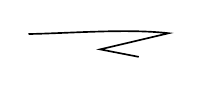
\begin{tikzpicture}[x=1cm,y=1cm]\draw[line width=.6pt] (0,.23) .. controls (.54,.24) and (1.25,.30) .. (1.78,.24) -- (.91,.035) -- (1.4,-.06);\end{tikzpicture}}

% lines 4–7
Reprenons l'exemple de la forme quadratique (21) et la forme $\varphi$ associée (22), d'où la structure d'algèbre de Lie (26) sur $E'$ de base $X=e'_1$, $Y=e'_2$, $H=e'_3$, et

% lines 8
\[
\omega'=-X\wedge H\wedge Y \tag*{(61)}
\]

% lines 9–11
(\inserted{Au lieu de $\omega$} on aurait pu choisir \inserted{\unsure{carrément}} $\omega'=-\omega=X\wedge H\wedge Y$ sans inconvénient, on aurait toujours une structure orthogonale spéciale $(q,\omega')\ \ldots$)

% lines 12–13
Explicitons alors par calcul toutes les opérations précédentes. On posera aussi

% lines 14
\[
\widetilde X=e_2,\quad\widetilde Y=e_1,\quad\widetilde H=e_3 \tag*{(62)}
\]

% lines 15–18
\deleted{or} et quand on regardera $E$ $(\simeq\mathscr O_S^3)$ comme une Algèbre de Lie, nous \unsure{préférerons|préfixerons|préférons} ces notations pour la base, qu'on prendra dans l'ordre

% lines 19
\[
\widetilde X,\ \widetilde H,\ \widetilde Y \tag*{(63)}
\]

% lines 20–22
\[
\text{\deleted{donc}}\quad\omega=\deleted{\unsure{-}}\widetilde X\wedge\widetilde H\wedge\widetilde Y
\quad\text{(\uline{NB} il n'y a pas de signe $-$ ici !)} \tag*{(64)}
\]

% lines 23
On trouve

% lines 24
\[
f(\widetilde X)=X,\ f(\widetilde Y)=Y,\quad f(\widetilde H)=2H \tag*{(65)}
\]

% lines 25
Ici, en vertu de (32)

% lines 26
\[
\Delta=\deleted{\unsure{2}}-2
\]

% lines 27
d'où on trouve

% lines foot
% archive sheet number: 18
\scanpage{20}
% lines 1
\[
f'(X)=2\widetilde X,\ f'(Y)=2(\widetilde Y),\ f'(H)=\widetilde H \tag*{(66)}
\]

% lines 2
La forme bilinéaire \deleted{associée} \inserted{$\varphi'$ correspondante sur $E'$} est donc définie par

% lines 3–4
\[
\left\{\begin{aligned}
\varphi'(\deleted{\unsure{\widetilde X}}X,X)=\varphi'(Y,Y)&=0 &\varphi'(H,H)&=1\\
\varphi'(X,\deleted{\unsure{Y}}H)=\varphi'(Y,H)&=0 &\varphi'(X,Y)&=2
\end{aligned}\right. \tag*{(67)}
\]

% lines 5–7
\[
\begin{aligned}
&\text{i.e. en termes de \unsure{v|$\eta$}}\\
\eta&=x\overset{\unsure{\leftrightarrow|\frown}}{X+h}H+yY\\
\eta'&=x'X+h'H+y'Y
\end{aligned}
\]

% lines 8
la forme $\varphi'$ s'explicite par

% lines 9
\[
\varphi'(\eta,\eta')=\varphi((x,h,y);(x',h',y'))=hh'+2(xy'+yx') \tag*{(68)}
\]

% lines 10–11
la forme quadratique associée $q'$ étant donnée par

% lines 12
\[
q'(\eta)=\varphi'(\eta,\eta)=h^2+4xy \tag*{(69)}
\]

% lines 13–16
\deleted{``En \unsure{général}''} \inserted{Si 2 non inv dans $S$} $\varphi'$ n'est pas associée à une forme quadratique, \deleted{en particulier en car.} car en car. 2 la forme $q'(\eta)$ se réduit à $h^2$, qui est non nulle\ldots

% lines 16–25
On notera que dans les coordonnées universelles choisie, permettant d'exprimer $q,\varphi,q',\varphi'$ \deleted{en} termes de \inserted{quatre} expressions \unsure{polynômiales|polynomiales} à coefficients entiers, aucune de ces expressions n'est divisible par un entier $>1$ -- i.e. les coeff. sont premiers entre eux. Cela signifi aussi que \deleted{au dessus de \unsure{n'importe} \unsure{ou}} \inserted{si $S$ est le spectre d'un corps} (de car. quelc.), ces quatre fonctions sont $\ne0$.

% lines foot
% archive sheet number: 19
\scanpage{21}
% lines 1–2
Calculant la loi de crochet sur $E$, on trouve

% lines 3
\[
\deleted{\unsure{X},}[\widetilde H,\widetilde X]=2\widetilde X,\ [\widetilde H,\widetilde Y]=-2\widetilde Y,\ [\widetilde X,\widetilde Y]=\widetilde H \tag*{(70)}
\]

% lines 4–8
qui est la loi bien connue du crochet de l'algèbre de Lie $\mathfrak{sl}(2)_S$ spéciale linéaire, qui est l'algèbre de Lie de $\mathrm{SL}(2)_S$. Quant à $f$, c'est l'homomorphisme d'Algèbres de Lie correspondant à l'\deleted{\unsure{hom|homom.}} \inserted{isogénie} bien connue

% lines 9
\[
\mathrm{SL}(2)_S\ \unsure{\mathbin{-}|\longrightarrow}\ \mathrm{GP}(1)_S \tag*{(71)}
\]

% lines 10–16
\deleted{qui \unsure{fa|f}} de noyau $\mu_2$ \inserted{(qui est le centre de $\mathrm{SL}(2)_S$)}. Quant à l'opération de $E'$ sur $E$, elle correspond à l'opération bien connue de $\mathrm{GP}(1)_S$ sur $\mathfrak{sl}(2)_S$, déduite par passage au quotient \deleted{\unsure{p}}de la représentation adjointe de $\mathrm{GL}(2)$ sur lui-= (qui est bien triviale sur le centre $\mu_2\ldots$). En termes des bases précédentes, on aura

% lines 17
\deleted{(71) $\rho_X=\widetilde\rho$}

% lines 18–20
\[
\left\{\begin{aligned}
\rho_E(X)=\widetilde\rho_E(\widetilde X):\quad&
\widetilde X\mapsto0,\ \widetilde Y\longmapsto\widetilde H,\ \widetilde H\longmapsto-2\widetilde X\\
\rho_E(Y)=\widetilde\rho_E(\widetilde Y):\quad&
\widetilde X\mapsto-\widetilde H,\ \widetilde Y\mapsto0,\ \widetilde H\mapsto2\widetilde Y\\
\rho_E(H)\ (=\tfrac12\widetilde\rho_{\widetilde H}\ \text{sic}):\quad&
\widetilde X\to\widetilde X,\ \widetilde Y\mapsto-\widetilde Y,\ \widetilde H\mapsto0
\end{aligned}\right. \tag*{(72)}
\]

% lines 21–22
(ici le plus commode était d'utiliser la ``formule oubliée'' (56 bis) \ldots)

% lines foot
% archive sheet number: 20
\scanpage{22}
% lines 1–8
\uline{Remarque} Si 2 inv. sur $S$, alors $f$ est un isomorphisme d'algèbres de Lie, \deleted{$\unsure{\rho_E|f}$} permettant d'identifier $E$ et $E'$ (c'est aussi l'identification habituelle d'un espace quadratique et de son dual), et $\rho_E$ est identifié à $\rho_{E'}$ ou à $\widetilde\rho_E$ ou $\widetilde\rho_{E'}\ldots$ ; $f'$ (qui s'identifie à $2\operatorname{id}_E$) n'a alors guère d'intérêt ! (Ces constatations s'appliquent plus général\textsuperscript{t} chaque fois que $\Delta$ est inv.)

% lines 9–14
Si par contre 2 est nul sur $S$, alors $f$ a comme noyau $\mathscr O_S\mathbin{.}\widetilde H$, qui est alors le \uline{centre} de $E=\mathfrak{sl}(2)$. Quant à $f'$, il a comme noyau $\mathscr O_S X\oplus\mathscr O_S Y$, qui est \deleted{aussi} \inserted{alors} l'Algèbre \uline{dérivée} de $E'=\mathfrak{gp}(1)$, \deleted{et \unsure{comme}} \inserted{qui} est aussi l'image de $f$, alors que l'image

% lines 14a
% slanted
\margin{\uline{NB} $\varphi$ alternée, sa connaissance ne permet pas de retrouver $q$ ; $\varphi'$ \uline{n'est pas} alternée (\unsure{i.e.|resp.} $q'$ n'est pas nulle, comme on l'a déjà \unsure{noté}\ldots).}

% lines 15–19
de $f'$ est le noyau $\mathscr O_S\widetilde H$ de $f$. [Par contre le centre de $\mathfrak{gp}(1)$ est nul -- c'est vrai sur tte base $S$, comme on vérifie facilement $\}$ -- tandis que le \unsure{groupe|gpe} dérivé de $\mathfrak{sl}(2).$ est égal au centre $\mathscr O_S\mathbin{.}\widetilde H$] Ici

% lines 20–24
l'existence de $f'$ (cf plus bas un contexte général) peut avoir un intérêt \ldots. Il faudrait par la suite expliciter la structure des formes de $\mathfrak s=\mathfrak{sl}(2)$ et $\mathfrak g=\mathfrak{gp}(1)$ en car. 2, et se convaincre qu'elle est trop triviale pour offrir

% lines foot
% archive sheet number: 21
\scanpage{23}
% lines 1–3
un intérêt (contrairement aux formes de $\mathrm{SL}(2)_S$ ou $\mathrm{GP}(1)_S$, qui sont équivalentes et équivalent aux formes de $\mathbb P^1_S\ldots$).

% lines 4–6
Revenant au cas général, il peut être intéressant de calculer la forme \deleted{\inserted{quadratique}} de Casimir de $\mathfrak g=E'$ et $\mathfrak s=E$, \unsure{définis|définies} par

% lines 7
\[
\deleted{\operatorname{Cas}_{E}(\unsure{\eta',\eta'|x,y})=\rho_{E'}\operatorname{Tr}\rho_E}
\tag*{\deleted{(73)}}
\]

% lines 8–9
\[
\deleted{\left\{\begin{aligned}
\operatorname{Cas}_{\unsure{\mathfrak g'|E'}}(x')\deleted{\unsure{,y'}})&=\operatorname{Tr}\rho_{E'}(x')^2\\
\operatorname{Cas}_E(x)&=\operatorname{Tr}\widetilde\rho_E(x)^2
\end{aligned}\right.}
\tag*{\deleted{(73)}}
\]

% lines 10–11
\deleted{(les formes bil. associées sont respectivement $2\operatorname{Tr}\rho_{E'}(x')\rho_{E'}(y')$ et $2\operatorname{Tr}\widetilde\rho_E(x)\widetilde\rho_E(y)$).}

% lines 12
\deleted{Le calcul donne :}

% lines 13
\[
\deleted{\operatorname{Cas}_E(x^{\unsure{'}})=\Delta\varphi\overset{\deleted{\unsure{x',x'|x,x}}}{(x,x)}} \tag*{\deleted{(74)}}
\]

% lines 14
\deleted{d'où, en remplaçant $(E,\omega,\varphi)$ par $(E',\omega',\varphi')$}

% lines 15
\[
\deleted{\operatorname{Cas}_E(x)=} \tag*{\deleted{(75)}}
\]

% lines 16–17
\[
\left\{\begin{aligned}
\operatorname{Cas}_{E'}(x',y')&=\operatorname{Tr}\bigl(\rho_{E'}(x')\mathbin{.}\rho_{E'}\unsure{(}y')\bigr)\\
\operatorname{Cas}_{E}(x,y)&=\operatorname{Tr}\bigl(\widetilde\rho_E(x)\mathbin{.}\widetilde\rho_E(y)\bigr)
\end{aligned}\right. \tag*{(73)}
\]

% lines 18
On trouve alors

% lines 19–20
\[
\left\{\begin{aligned}
\operatorname{Cas}_{E'}(x',y')&=2\varphi'(x',y')\\
\operatorname{Cas}_E(x,y)&=-2\Delta\varphi(x,y)
\end{aligned}\right. \tag*{(74)}
\]

% lines 21–23
Pour le voir, on note d'abord que les \inserted{deux} formules ont la propriété d'homogénéité qu'il faut, quand on multiplie $\omega$ par $\lambda$, $\varphi$ par $\mu$ : les

% lines foot
% archive sheet number: 22
\scanpage{24}
% lines 1–4
\uline{deux} mbs de la $1^{\mathrm{ère}}$ sont multipliés alors par $(\mu\lambda)^2=\mu^2\lambda^2$, et les \uline{deux} mbs de la seconde par $(\mu^2\lambda)^2=\mu^4\lambda^2$. On vérifie ensuite les formules dans le cas particulier (21).

% lines 4–11
On peut se simplifier le travail en notant que pour l'une et l'autre formule, les deux mbs sont des formes invariantes sous l'action du groupe \inserted{spécial} orthogonal $\underline{\mathrm O}(q,\omega)$ (sur $\operatorname{Spec}\unsure{Z|\mathbb Z|\mathbf Z}$ si on veut) or il n'y a (en car zéro, si on y tient -- celà suffit -- qu' une seule forme invariante sym, à scalaire près, ce qui montre la proportionnalité.

% lines 11–16
Pour avoir le coefficient correctif, il suffit de calculer la valeur des 2 mbs pour un couple d'arguments pour lesquels ils soient non nuls, p.ex. $x'=y'=H$, $x=y=\widetilde H$. On trouve

% lines 17–22
\[
\begin{aligned}
\operatorname{Cas}_{E'}(H,H)&=1+1+0=2\\
\varphi'(H,H)&=1\\
\operatorname{Cas}_E(\widetilde H,\widetilde H)
&=\operatorname{Cas}_{E'}(2H,2H)=4\operatorname{Cas}_{E'}(H,H)=8\\
&\quad(\text{ou encore }=4+4+0)\\
\varphi(\widetilde H,\widetilde H)&=2\\
\Delta&=-2
\end{aligned}
\]

% lines 23–26
On note qu'en vertu du \deleted{\unsure{bon|beau|bref}} principe de conservation des identités polynômiales, il suffit de prouver (74) sur un corps de car. 0 alg. clos, \deleted{mais \unsure{alors} on \unsure{peut}} \inserted{avec $f$ un iso i.e.} $\varphi$ associée

% lines foot
% archive sheet number: 23
\scanpage{25}
% lines 1–6
à une forme quadratique non dég -- qu'on peut dès lors, pour une base convenable, mettre sous la forme $xy+z^2$. Quitte à multiplier $\omega$ par un scalaire (ce qui est loisible) on peut supposer que $\omega=e_1\wedge e_2\wedge e_3$, ce qui nous ramène au cas déjà traité.

% lines 7–9
Lorsque $\varphi$ est associé à une forme quadratique $q$, on tire de la deuxième formule (74), compte tenu de $\varphi(x,x)=2q(x)$ :

% lines 10
\[
\operatorname{Cas}_E(x,x)=-2\Delta\varphi(x,x)=-4\Delta q(x) \tag*{(75)}
\]

% lines 11–12
ce qui, dans le cas d'une forme \inserted{$q$} spéciale orthogonale pour $\omega$, d'où $\Delta=-2$, donne

% lines 13
\[
\operatorname{Cas}_E(x,x)=8q(x) \tag*{(76)}
\]

% lines 14–17
Donc dans ce cas, \deleted{\unsure{on a}} si 2 est inv, (ou plus gén. non div. de 0) $q(x)$ se \uline{déduit} de la structure d'algèbre de Lie sur $E$, comme l'\unsure{op.|exp.|opér.} de Casimir divisé par $8\ldots$

% lines 18–19
On \unsure{tire|tirera|trouve} de =, par la première formule

% lines 20
\[
\operatorname{Cas}_{E'}(x',x')=2\varphi'(x',x')=2q'(x') \tag*{\deleted{\unsure{(77)}}(77)}
\]

% lines 21–24
i.e. on retrouve la forme quadratique $q'(x')$ (ou la forme bil $\varphi'$ dont elle provient) à l'aide de la structure d'Algèbre de Lie de $E'_{\deleted{\unsure{\mathfrak g}}}=\mathfrak g$.

% lines foot
% archive sheet number: 24
\scanpage{26}
% lines 1–4
Remarques (devrait venir avec observations après formule (42)). Le crochet $[\ ,\ ]_{\varphi\unsure{*|'|{}}}\inserted{=[\ ,\ ]_{\varphi,\omega}}$ sur $E'$ est multiplié par $\lambda\mu$ si $\omega$ est multiplié par $\lambda$, $\varphi$ par $\mu$ ; \deleted{on a en effet}

% lines 5–6
\[
\left\{\begin{aligned}
[\ ,\ ]_{\lambda\omega,\mu\varphi}&=\lambda\mu[\ ,\ ]_{\omega,\varphi}\\
[\ ,\ ]_{\lambda\omega,(\mu\varphi)'}&=\lambda\mu^2[\ ,\ ]_{\omega,\varphi'}
\end{aligned}\right. \tag*{(78)}
\]

% lines 7
On en conclut que

% lines 8
\[
[\ ,\ ]_{\omega,\varphi}=[\ ,\ ]_{\omega_1,\varphi_1}
\Longleftrightarrow\inserted{\exists\lambda\in\Gamma(\unsure{S|s},\mathscr O_S^{\unsure{*|\times}})}
\ \omega_1=\lambda\omega,\ \varphi_1=\lambda^{-1}\varphi \tag*{(79)}
\]

% lines 9–12
\deleted{D'autre part} (compte tenu que pour $\omega$ fixé, la corr. entre $\varphi$ et $[\ \ ]_\varphi$ est biunivoque). D'autre part, \uline{si} $\det(f)=\delta(\varphi)$ \uline{inversible} i.e. $f$ iso, \inserted{et pour $\omega$ fixé} alors

% lines 13–14
$f\longmapsto f'=\alpha'_\omega\circ\bigwedge^2 f\circ\alpha_\omega^{-1}$ est \inserted{presque} bijectif, \deleted{\unsure{en effet}} \inserted{de façon} plus précise si $f,g:E\mathbin{-}E'$, on a

% lines 15–16
\[
f'=g'\Longleftrightarrow g=\varepsilon f,\quad
\varepsilon\in\Gamma(S,\mu_2)\ \text{i.e.}\ \varepsilon^2=1 \tag*{(80)}
\]

% lines 17–18
[car $f'=g'\Rightarrow\Delta(f\unsure{'|{}})=\Delta(g')$ i.e. $\Delta(f)^2=\Delta(g)^2$ i.e. $\Delta(g)=\varepsilon\Delta(f)$, d'où compte tenu de

% lines 19
\[
f=\Delta(f)^{-1}(f')',\quad g=\Delta(g)^{-1}(g')'\quad g=\varepsilon f\quad]
\]

% lines 19–20
On en déduit aisément que

% lines 21–24
\[
\begin{aligned}
[\ ,\ ]_{\omega_1,(\varphi_1)'}=[\ ,\ ]_{\omega,(\varphi)'}&\Longleftrightarrow\omega_1=\lambda\omega,\ \varphi_1=\mu\varphi\\
&\text{avec }\lambda\mu^2=1\ \text{i.e.}\\
&\mu\ \text{\uline{une} racine carrée}\\
&\text{de }\lambda^{-1}
\end{aligned} \tag*{(81)}
\]

% lines 25
(\uline{NB} $\lambda$ et $\mu$ uniquement déterminés).

% lines foot
% archive sheet number: 25
\scanpage{27}
% lines 1–7
En car. 2, la catégorie des formes de $\mathfrak{sl}(2)$ est équivalente à celle des couples $(V,E)$ où $V$ est un Module vectoriel de rang 2 et $E$ une extension de \deleted{$\unsure{E}$} $V$ par $\det V$ (\uline{NB} pour $V$ fixé, la donnée d'une telle extension équivaut à celle d'une \deleted{\unsure{fibré}} extension de $\det V^{-1}$ par $\unsure{\check V^*|\check V}$ ou de $\mathscr O_S$ par $(\det V)\otimes\check V\simeq V$, i.e. à la cat. des fibrés affines sous $V\ldots$).

% lines 7–12
La catégorie des formes de $\mathfrak{gp}(1)$ équivaut à celle des \deleted{\unsure{extens}} couples $(V',E')$ d'un Module vectoriel \inserted{$V'$} de rang 2, et d'une extension \inserted{$E'$} de $\mathscr O_S$ par $V'$ ; (pour $V'$ fixé, la cat équivaut à celle des fibrés affines sous $V'$).

% lines 12–14
Disons que deux telles algèbres de Lie \inserted{$E,E'$} sont accouplées si on a un accouplement dualisant entre $E,E'$, dans

% lines 15–16
\diagram{\begin{tikzcd}[ampersand replacement=\&,column sep=small,row sep=small]
\& \mathscr O_S \arrow[d,phantom,"\rotatebox{90}{$\simeq$}" description] \& \& \& \\
\unsure{\bullet|0} \arrow[r,no head] \& \det V \arrow[r,no head] \& E \arrow[r] \& V \arrow[r] \& 0\\
\bullet \arrow[r,no head] \& \deleted{\unsure{\det}}\mathscr O_S \& E' \arrow[l] \& \deleted{\unsure{\check{\phantom V}}}V' \arrow[l] \arrow[d,phantom,"\rotatebox{90}{$\simeq$}" description] \& \bullet \arrow[l]\\
\& \& \& V \&
\end{tikzcd}}

% lines 15–20
lequel le sous-module $\det V$ de $E$ est l'orthogonal du sous module $V'$ de $E'$ -- qui est donc \deleted{iso à $\check V$ =} dual de $V$, et de = $\det V$ est dual de $\mathscr O_S$, donc can. iso. à $\mathscr O_S$. \deleted{Donc} $V$ est en fait muni d'une structure symplectique, \deleted{et} \inserted{par laquelle} $V'\simeq V$.

% lines 20–26
La catégorie des couples \inserted{accouplés} de formes de $\mathfrak{sl}(2),\mathfrak{gp}(1)$ est donc équivalente à celle des triples $(V,\varphi,E)$ d'un Module vectoriel $V$ de rang 2, avec structure symplectique $\varphi$ et ext. de $V$ par $\mathscr O_S$ (ce qui revient à ext. de $\mathscr O_S$ par $\check V\simeq V$, ou encore fibré affine sous $V$) : c'est donc équivalent

% lines foot
% archive sheet number: 26
\scanpage{28}
% lines 1–6
à la donnée d'un fibré en ``plans affines symplectiques'' (ou unimodulaires). Le \inserted{\unsure{schém. en|schéma en}} groupes des autom. d'une telle structure est donc le produit $1/2$ direct de $\underline{\mathrm{SL}}(V)$ et de $\underline V$ -- lisse de dim 5 -- ce n'est en tous cas pas \deleted{\unsure{le}} une forme de $\mathrm{GP}(1)$ !

% lines 6–9
Le groupe des autom. \deleted{\unsure{de}}d'une forme de $\mathfrak{sl}(2)$ ou $\mathfrak{gp}(1)$ est $\simeq$ groupe affine à deux variables, lisse de dim rel. 6.

% lines 10–12
On déduit aisément, de la structure précédente, les données $f,f',\rho_{E'}$. En effet, $f$ est le composé

% lines 12
\diagram{\begin{tikzcd}[ampersand replacement=\&,column sep=small]
E \arrow[r,"\mathrm{can}"] \& V \arrow[r,"\varphi"] \& V' \arrow[r,"\mathrm{can}"] \& E',
\end{tikzcd}}

% lines 12–13
$f'$ est le composé

% lines 13
\diagram{\begin{tikzcd}[ampersand replacement=\&,column sep=small]
E' \arrow[r,"\mathrm{can}"] \& \mathscr O_S \arrow[r,no head,"\varphi" description] \& \det V \arrow[r,"\mathrm{can}"] \& E,
\end{tikzcd}}

% lines 13–15
enfin $\rho_{E'}$ \inserted{(op. de $E'$ sur $E$)} est l'opération \deleted{qui sur $V'=f(E)$ se} \inserted{contragrédiente de l'op. adjointe de $E'$} \ldots.

% lines 15–19
\deleted{\unsure{déduit} de la représentation adjointe de $E$, qui est nulle sur $\det V=\mathscr O_S\subset E$, et qui pour un $H\in E'$ au dessus de 1 donne l'opération $\rho_{E'}(H):E\mathbin{-}E$ qui (étant nulle sur $\det V=\mathscr O_S$) se factorise en \deleted{\unsure{le}}\inserted{un} splitting}

% lines foot
% archive sheet number: 27
\scanpage{29}
% lines 1–3
Soit $q$ forme quadratique lisse sur $E$, $\varphi$ la forme bilinéaire associée, $\omega$ \deleted{\unsure{$\in$}} une base de $\underline{\det} E$ telle que

% lines 4
\[
\delta'(q)=-\omega^{\otimes(-2)} \tag*{(82)}
\]

% lines 5
Posons

% lines 6
\[
G'=\underline{\mathrm{SO}}(q)=\underline{\operatorname{Aut}}(E,q,\omega) \tag*{(83)}
\]

% lines 7–10
Soit $\widetilde G$ le \deleted{centre de $G$, canoniquement} \inserted{``revêtement simplement connexe'' de $G$, $\mathfrak z$ le noyau} de $\widetilde G^{\deleted{\unsure{'|\mathfrak z}}}\to G$, canoniquement isomorphe à $\mu_2$ \deleted{(correspondant aux homothéties de carré 1) posons} \inserted{d'où}

% lines 11
\diagram{(84)\quad\begin{tikzcd}[ampersand replacement=\&,column sep=small]
1 \arrow[r,no head] \& \mu_2 \arrow[r] \& \widetilde G^{\deleted{\unsure{'|+}}} \arrow[r,"F"] \& G\deleted{\unsure{/\mathfrak z|\mathfrak z}} \arrow[r] \& 1
\end{tikzcd}}

% lines 12
Soient

% lines 13–14
\[
\left\{\begin{aligned}
\mathfrak s&=\underline{\operatorname{Lie}}(\widetilde G)\\
\mathfrak g&=\underline{\operatorname{Lie}}(G)
\end{aligned}\right. \tag*{(85)}
\]

% lines 15
Alors on a un hom can (épim. de noyau $\mathfrak z$)

% lines 16
\diagram{(86)\quad\begin{tikzcd}[ampersand replacement=\&]
F\colon \widetilde G \arrow[r] \& G
\end{tikzcd}}

% lines 17–19
et une opération (obtenue par passage au quotient dans la représentation adjointe de $\widetilde G$ sur lui =

% lines 20
\diagram{(87)\quad\begin{tikzcd}[ampersand replacement=\&]
G^{\deleted{\unsure{\sim}}\deleted{'}} \arrow[r,"\rho"] \& \underline{\operatorname{Aut}}_{S\text{-gr}}(\widetilde G)
\end{tikzcd}}

% lines 21
rendant commutatif le diagramme

% lines 22–24
\diagram{(88)\quad\begin{tikzcd}[ampersand replacement=\&,column sep=small,row sep=large]
\widetilde G \arrow[r,"F"] \arrow[dr,"\mathrm{ad}_{\widetilde G}"'] \& G^{\deleted{'}} \arrow[d,"\rho"] \arrow[dr,"\mathrm{ad}_{G^{\deleted{'}}}"] \& {}\\
{} \& \underline{\operatorname{Aut}}_{S\text{-gr}}(\widetilde G)
\arrow[r,"\substack{\text{passage}\\\text{au quotient}}"'] \& \underline{\operatorname{Aut}}_{S\text{-gr}}(G)
\end{tikzcd}}

% lines foot
% archive sheet number: 28
\scanpage{30}
% lines 1–2
ou ce qui revient au même, on a comm. dans

% lines 3–5
\diagram{(89)\quad\begin{tikzcd}[ampersand replacement=\&,row sep=large]
\widetilde G\times\widetilde G \arrow[r,"\mathrm{ad}_{\widetilde G}"] \arrow[d,"F\times\operatorname{id}_G"'] \& \widetilde G \arrow[d,"1"]\\
G^{\deleted{\unsure{'|+}}}\times\widetilde G \arrow[r,"\rho"] \arrow[d,"\operatorname{id}_{G'}\times F"'] \& \widetilde{\deleted{\unsure{G}}G} \arrow[d,"F"]\\
G^{\deleted{'}}\times G^{\deleted{'}} \arrow[r,"\mathrm{ad}_{G^{\deleted{'}}}"] \& G^{\deleted{'}}
\end{tikzcd}}

% lines 6
En passant aux Algèbres de Lie, on aura

% lines 7
\diagram{(90)\quad\begin{tikzcd}[ampersand replacement=\&]
\mathfrak s \arrow[r,"\deleted{\unsure{d}}f_{\mathfrak s}"] \& \mathfrak g
\end{tikzcd}\quad hom d'alg. de Lie}

% lines 8
et une opération

% lines 9
\diagram{(91)\quad\begin{tikzcd}[ampersand replacement=\&]
\mathfrak g \arrow[r,"\rho_{\mathfrak g}"] \& \underline{\operatorname{Dér}}(\mathfrak s)
\end{tikzcd}}

% lines 10
rendant commutatif le diagramme

% lines 11–13
\diagram{(92)\quad\(\left\{\vcenter{\hbox{\begin{tikzcd}[ampersand replacement=\&,row sep=large]
\deleted{\mathfrak g\times}\ \mathfrak s\times\mathfrak s \arrow[r,"\mathrm{ad}_{\mathfrak s}"] \arrow[d,"(f_{\mathfrak s}\times\mathfrak s)"'] \& \mathfrak s \arrow[d,"1"]\\
\mathfrak g\mathbin{\unsure{\wedge|\times}}\mathfrak s \arrow[r] \arrow[d] \& \mathfrak s \arrow[d,"f_{\mathfrak s}"]\\
\mathfrak g\times\mathfrak g \arrow[r,"\mathrm{ad}_{\mathfrak g}"] \& \mathfrak g
\end{tikzcd}}}\right.\)}

% lines 14–15
\deleted{\unsure{Enfin, le|Remarques}} Ceci posé, on va définir des isom. canoniques de Modules :

% lines 16–17
\diagram{(93)\quad\(\left\{\vcenter{\hbox{\begin{tikzcd}[ampersand replacement=\&,row sep=small]
E \arrow[r,"{\overset{i}{\sim}}"] \& \mathfrak s\\
E' \arrow[r,"{\overset{j}{\sim}}"] \& \mathfrak g
\end{tikzcd}}}\right.\)}

% lines 18–19
\deleted{qui soit} Transportant par \unsure{ses|ces} isom. les lois $[\ ,\ ]$ sur $\mathfrak s$ et $\mathfrak g$, \deleted{\unsure{le|et}} $f_{\mathfrak s}:\mathfrak s\unsure{\mathbin{-}|\to}\mathfrak g$

% lines foot
% archive sheet number: 29
\scanpage{31}
% lines 1–3
et $\rho_{\mathfrak g}:\mathfrak g\longrightarrow\operatorname{Dér}(\mathfrak s)$, on trouve respectivement : la loi $[\ ,\ ]_{\varphi'}$ sur $E$, la loi $[\ ,\ ]_{\varphi}$ sur $E'$\unsure{,}, l'application $f:\inserted{E\to E'}$, l'hom $\rho_E$.

% lines 4
Enfin, l'hom. composé

% lines 5
\diagram{\begin{tikzcd}[ampersand replacement=\&,column sep=small]
\mathfrak g \arrow[r,"{\rho_{\mathfrak g}^{\deleted{\unsure{\mathrm{ad}}}}}"] \& \underline{\operatorname{Dér}}(\mathfrak s) \arrow[r,"\sim","(i)"'] \& \underline{\operatorname{Dér}}(E) \arrow[r,no head] \& \underline{\operatorname{End}}(E)
\end{tikzcd}}

% lines 6–8
n'est autre que la repr. linéaire de $\mathfrak s=\underline{\operatorname{Lie}}(\unsure{G|G'})$ correspondant à la repr. \deleted{\unsure{taut|fond}}\unsure{tautologique} de $G$ sur $E$.

% lines 9–10
\uline{Construction} Considérons $E'$ avec la loi $[\ ,\ ]_{\varphi\unsure{*|'|{}}}$, on sait que $E'$ opère sur $E$ par $\rho_{E'}$

% lines 11
\diagram{\begin{tikzcd}[ampersand replacement=\&]
E' \arrow[r] \& \underline{\operatorname{Dér}}(E,[\ ,\ ]_{\varphi'})
\end{tikzcd}}

% lines 12–15
en fait on sait que $E'$ s'envoie dans les endom. \inserted{de $E$} qui invarient infinitésimalement $q$, \inserted{\uline{et} qui invarient $\omega$} lesquels forment précisément l'algèbre de \uline{Lie} $\mathfrak g$ de $G$, d'où finalement un hom

% lines 16
\diagram{\begin{tikzcd}[ampersand replacement=\&]
E' \arrow[r,"j" description] \& \mathfrak g
\end{tikzcd}}

% lines 17–20
qui est compatible avec le crochet. Je dis \uline{que c'est un iso}. Comme $E'$ et $\mathfrak g$ sont \deleted{\unsure{des}} loc. \unsure{libre|libres} de rang 3, il suffit de prouver que c'est injectif sur chaque fibre \inserted{géom}, \unsure{ou|on}

% lines foot
% archive sheet number: 30
